% GNUPLOT: LaTeX picture with Postscript
\begingroup
  \makeatletter
  \providecommand\color[2][]{%
    \GenericError{(gnuplot) \space\space\space\@spaces}{%
      Package color not loaded in conjunction with
      terminal option `colourtext'%
    }{See the gnuplot documentation for explanation.%
    }{Either use 'blacktext' in gnuplot or load the package
      color.sty in LaTeX.}%
    \renewcommand\color[2][]{}%
  }%
  \providecommand\includegraphics[2][]{%
    \GenericError{(gnuplot) \space\space\space\@spaces}{%
      Package graphicx or graphics not loaded%
    }{See the gnuplot documentation for explanation.%
    }{The gnuplot epslatex terminal needs graphicx.sty or graphics.sty.}%
    \renewcommand\includegraphics[2][]{}%
  }%
  \providecommand\rotatebox[2]{#2}%
  \@ifundefined{ifGPcolor}{%
    \newif\ifGPcolor
    \GPcolortrue
  }{}%
  \@ifundefined{ifGPblacktext}{%
    \newif\ifGPblacktext
    \GPblacktexttrue
  }{}%
  % define a \g@addto@macro without @ in the name:
  \let\gplgaddtomacro\g@addto@macro
  % define empty templates for all commands taking text:
  \gdef\gplbacktext{}%
  \gdef\gplfronttext{}%
  \makeatother
  \ifGPblacktext
    % no textcolor at all
    \def\colorrgb#1{}%
    \def\colorgray#1{}%
  \else
    % gray or color?
    \ifGPcolor
      \def\colorrgb#1{\color[rgb]{#1}}%
      \def\colorgray#1{\color[gray]{#1}}%
      \expandafter\def\csname LTw\endcsname{\color{white}}%
      \expandafter\def\csname LTb\endcsname{\color{black}}%
      \expandafter\def\csname LTa\endcsname{\color{black}}%
      \expandafter\def\csname LT0\endcsname{\color[rgb]{1,0,0}}%
      \expandafter\def\csname LT1\endcsname{\color[rgb]{0,1,0}}%
      \expandafter\def\csname LT2\endcsname{\color[rgb]{0,0,1}}%
      \expandafter\def\csname LT3\endcsname{\color[rgb]{1,0,1}}%
      \expandafter\def\csname LT4\endcsname{\color[rgb]{0,1,1}}%
      \expandafter\def\csname LT5\endcsname{\color[rgb]{1,1,0}}%
      \expandafter\def\csname LT6\endcsname{\color[rgb]{0,0,0}}%
      \expandafter\def\csname LT7\endcsname{\color[rgb]{1,0.3,0}}%
      \expandafter\def\csname LT8\endcsname{\color[rgb]{0.5,0.5,0.5}}%
    \else
      % gray
      \def\colorrgb#1{\color{black}}%
      \def\colorgray#1{\color[gray]{#1}}%
      \expandafter\def\csname LTw\endcsname{\color{white}}%
      \expandafter\def\csname LTb\endcsname{\color{black}}%
      \expandafter\def\csname LTa\endcsname{\color{black}}%
      \expandafter\def\csname LT0\endcsname{\color{black}}%
      \expandafter\def\csname LT1\endcsname{\color{black}}%
      \expandafter\def\csname LT2\endcsname{\color{black}}%
      \expandafter\def\csname LT3\endcsname{\color{black}}%
      \expandafter\def\csname LT4\endcsname{\color{black}}%
      \expandafter\def\csname LT5\endcsname{\color{black}}%
      \expandafter\def\csname LT6\endcsname{\color{black}}%
      \expandafter\def\csname LT7\endcsname{\color{black}}%
      \expandafter\def\csname LT8\endcsname{\color{black}}%
    \fi
  \fi
    \setlength{\unitlength}{0.0500bp}%
    \ifx\gptboxheight\undefined%
      \newlength{\gptboxheight}%
      \newlength{\gptboxwidth}%
      \newsavebox{\gptboxtext}%
    \fi%
    \setlength{\fboxrule}{0.5pt}%
    \setlength{\fboxsep}{1pt}%
\begin{picture}(11520.00,8640.00)%
\definecolor{gpBackground}{rgb}{1.000, 1.000, 1.000}%
\put(0,0){\colorbox{gpBackground}{\makebox(11520.00,8640.00)[]{}}}%
    \gplgaddtomacro\gplbacktext{%
      \colorrgb{0.15,0.15,0.15}%%
      \put(543,593){\makebox(0,0)[r]{\strut{}0}}%
      \colorrgb{0.15,0.15,0.15}%%
      \put(543,1473){\makebox(0,0)[r]{\strut{}5}}%
      \colorrgb{0.15,0.15,0.15}%%
      \put(543,2354){\makebox(0,0)[r]{\strut{}10}}%
      \colorrgb{0.15,0.15,0.15}%%
      \put(543,3234){\makebox(0,0)[r]{\strut{}15}}%
      \colorrgb{0.15,0.15,0.15}%%
      \put(543,4115){\makebox(0,0)[r]{\strut{}20}}%
      \colorrgb{0.15,0.15,0.15}%%
      \put(543,4995){\makebox(0,0)[r]{\strut{}25}}%
      \colorrgb{0.15,0.15,0.15}%%
      \put(543,5876){\makebox(0,0)[r]{\strut{}30}}%
      \colorrgb{0.15,0.15,0.15}%%
      \put(543,6756){\makebox(0,0)[r]{\strut{}35}}%
      \colorrgb{0.15,0.15,0.15}%%
      \put(543,7637){\makebox(0,0)[r]{\strut{}40}}%
      \colorrgb{0.15,0.15,0.15}%%
      \put(645,409){\makebox(0,0){\strut{}0}}%
      \colorrgb{0.15,0.15,0.15}%%
      \put(1967,409){\makebox(0,0){\strut{}1000}}%
      \colorrgb{0.15,0.15,0.15}%%
      \put(3290,409){\makebox(0,0){\strut{}2000}}%
      \colorrgb{0.15,0.15,0.15}%%
      \put(4612,409){\makebox(0,0){\strut{}3000}}%
      \colorrgb{0.15,0.15,0.15}%%
      \put(5934,409){\makebox(0,0){\strut{}4000}}%
      \colorrgb{0.15,0.15,0.15}%%
      \put(7256,409){\makebox(0,0){\strut{}5000}}%
      \colorrgb{0.15,0.15,0.15}%%
      \put(8579,409){\makebox(0,0){\strut{}6000}}%
      \colorrgb{0.15,0.15,0.15}%%
      \put(9901,409){\makebox(0,0){\strut{}7000}}%
    }%
    \gplgaddtomacro\gplfronttext{%
      \colorrgb{0.15,0.15,0.15}%%
      \put(153,4524){\rotatebox{90}{\makebox(0,0){\strut{}Amplitud}}}%
      \colorrgb{0.15,0.15,0.15}%%
      \put(5929,130){\makebox(0,0){\strut{}Frecuencia [Hz]}}%
      \colorrgb{0.00,0.00,0.00}%%
      \put(7966,8292){\makebox(0,0)[l]{\strut{}Respuesta en frecuencia de la ventana}}%
      \colorrgb{0.00,0.00,0.00}%%
      \put(7966,8118){\makebox(0,0)[l]{\strut{}Respuesta del filtro de coefs LPC}}%
    }%
    \gplbacktext
    \put(0,0){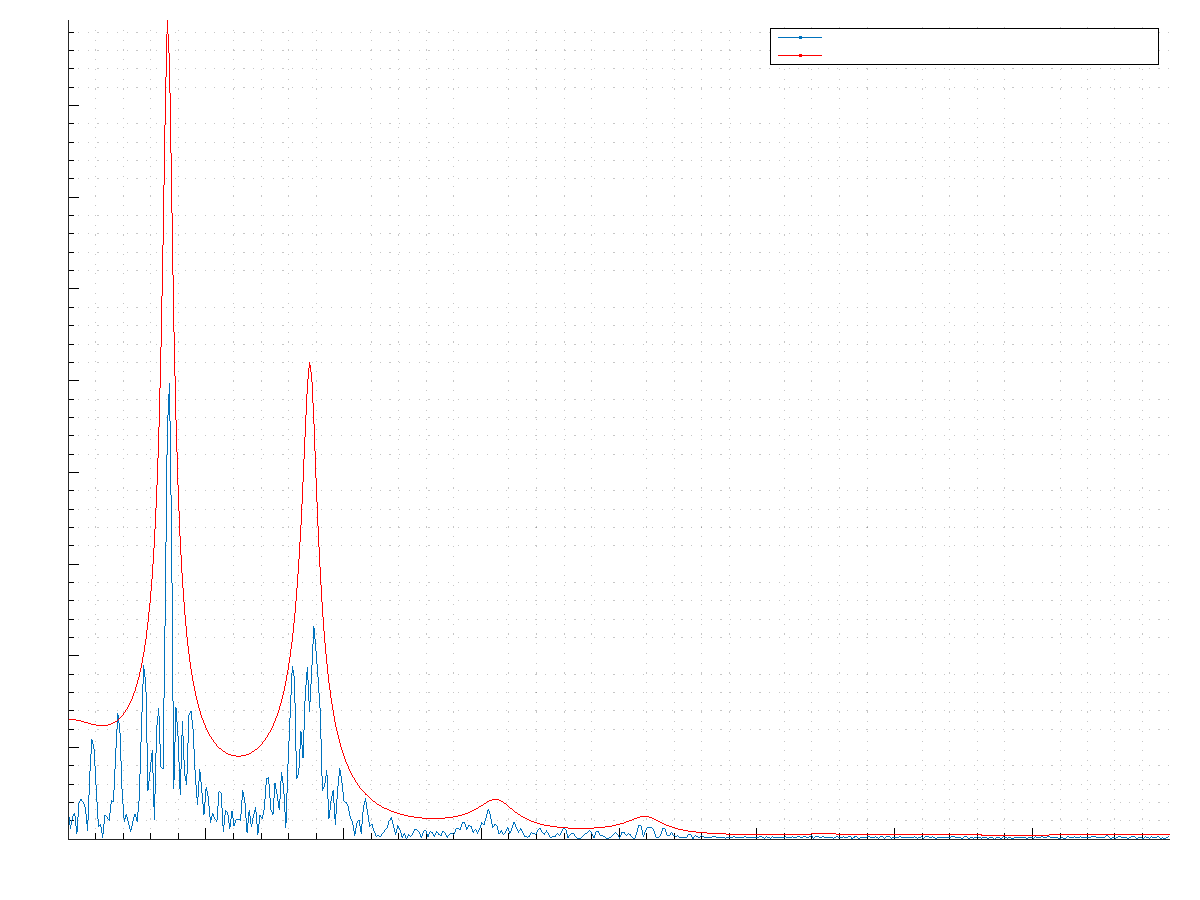
\includegraphics{./graf_envolvente}}%
    \gplfronttext
  \end{picture}%
\endgroup
